%!TEX root = main.tex
\section{Fixing Boundary Imperfections\label{precision}}
\subsection{Tile Data Model}
At the heart of our aggregation techniques is a \emph{tile data representation}. A tile is the smallest non-overlapping discrete unit created by overlaying all of the workers' segmentations on top of each other. %with a certain probability of being contained in the ground truth segmentation. 
The tile representation allows us to aggregate segmentations from multiple workers, rather than being restricted to a single worker's segmentation. This allows us to fix one worker's errors with help from another worker's segmentation. \changes{In Figure \ref{tile_demo} (right), we display three worker segmentations for a toy example. Worker 1's segmentation is represented in pink, worker 2's segmentation in yellow, and worker 3's segmentation in blue. These segmentations overlap resulting in a partitioning or tiling of the image with 6 distinct resulting tiles. For instance, tile $t_1$ is the portion of worker 1's segmentation that is not contained in worker 2 or worker 3's segmentations, tile $t_2$ is the intersection of all three workers' segmentations, and $t_3$ is the intersection of worker 2 and worker 3's segmentations excluding worker 1's segmentation. Any subset of these 6 tiles can contribute towards the final segmentation.}
\begin{figure}[h!]
\centering
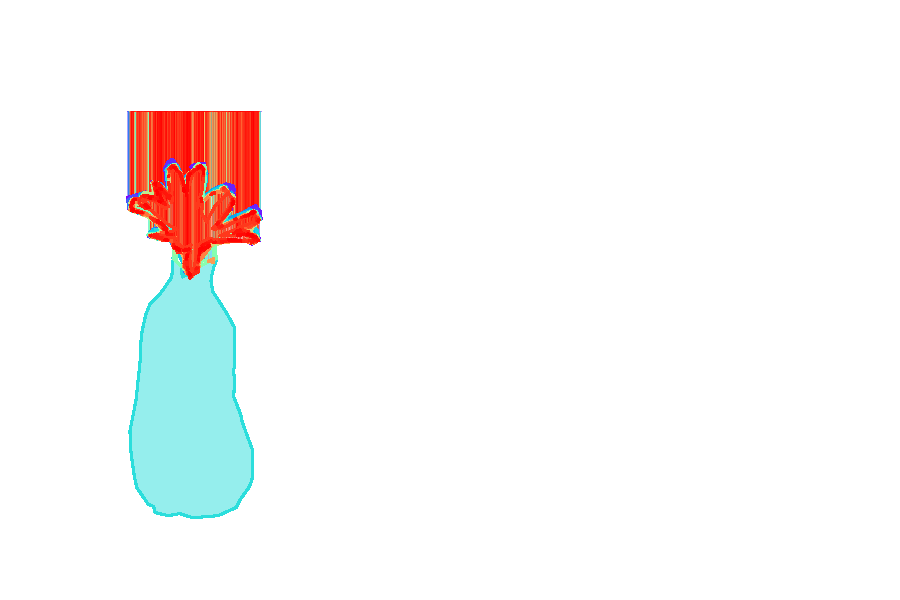
\includegraphics[width=0.85\linewidth]{plots/tile.pdf}
\caption{Left: Toy example demonstrating tiles created by three workers' segmentations around a dumbell object delineated by the black dotted line. Right: Segmentation boundaries drawn by five workers shown in red. Overlaid segmentation creates a mask where the color indicates the number of workers who voted for the tile region.}
\label{tile_demo}
% \setlength{\abovecaptionskip}{-15pt}
% \setlength{\belowcaptionskip}{-25pt}
\end{figure}  
%both worker 1 and 2's segmentation can contribute towards the final segmentation.
\par The simple but powerful idea of tiles also allows us to reformulate our problem from one of ``generating a segmentation'' to a setting that is much more familiar to crowdsourcing researchers. Since tiles are the lowest granularity units created by overlaying all workers' segmentations on top of each other, each tile is either completely contained within or outside a given worker segmentation. Specifically, we can regard a worker segmentation as multiple boolean responses where they have voted `yes' or `no' to every tile independently. Intuitively, a worker votes `yes' for every tile that is contained in their segmentation, and `no' for every tile that is not. As shown in Figure \ref{tile_demo} (right), tile $t_2$ is voted `yes' by worker 1, 2, and 3; tile $t_3$ is voted `yes' by worker 2 and 3. The goal of our aggregation algorithms is to pick an appropriate set of tiles that effectively trades off precision versus recall. This is equivalent to making a boolean decision of ``include tile in output'', or ``yes'' versus ``don't include tile in output'', or ``no'' for each tile, given multiple boolean worker votes for each tile.
Thus we have projected the original problem of generating a segmentation onto a boolean aggregation problem. We focus on algorithms for the boolean decision problem setting for the remainder of this section.

\subsection{Majority Vote Aggregation (MV)} 
\par \noindent Majority Vote aggregation is a standard technique for boolean aggregation in crowdsourcing. We treat each tile as an independent boolean decision and assign equal weight to each worker's votes, thereby implictly assuming that all workers are equal. We include a tile in the output segmentation if and only at least 50\% of all workers have voted ``yes'' for the tile. In practice, however, not all workers are equal---some workers tend to make more mistakes than others, or have particular biases. Furthermore, not all tile decisions are necessarily independent because our aggregate decisions on some tiles could affect our belief of worker qualities, which in turn could influence our aggregation decisions on other tiles. Next, we extend our approach to capture and incorporate worker qualities into our algorithms.

\subsection{Worker Quality-Aware Algorithms}
\techreport{
    One way to think about the majority vote algorithm is to say that it selects all tiles that have at least a 50\% probability of being part of the ground truth segmentation, where the fraction of workers that have voted ``yes'' for a tile is an approximation for the probability that a tile belongs in the ground truth segmentation. In this section we formalize the notion of the probability, or {\em likelihood} of a tile belonging in the ground truth. Since some workers are more accurate than others, the likelihood of a tile should depend not only on the votes of workers, but also on the ``qualities'' of the participating workers. It should be noted that do not distinguish between pixels within a tile, i.e., for any given tile we either include all its constituent pixels in our output, or exclude all of them. We model worker qualities based on their probabilities of getting different pixels correct.
}

We intuitively describe three worker models that we experiment with below.
\papertext{In our technical report, we formalize the notion of the probability that a set of tiles forms the ground truth, and solve the corresponding maximum likelihood problem, for each of these worker models.}

\subheading{Worker quality models.}
% Tiles are finer grained than bounding boxes. Our tile-based approach is inspired by the S-T graph in the classical graph cut problem, where the goal of image segmentation is to find a vertex partition between the object and background regions.
Let us first define some useful notation.
\par Let $\mathcal{T}=\{t_k\}$ be the set of all non-overlapping tiles for an object $i$. T is the ground truth tile set. $T^\prime$ is some combination of tiles chosen from $\mathcal{T}$.
 The indicator label $l_{kj}$ is one when worker j votes on the tile $t_{k}$ (i.e. the bounding box that he draws contains $t_{k}$), and zero otherwise. The indicator matrix consisting of tile indicator for all workers is denoted as $\mathbf{l_{kj}}$.

\par We propose three different worker error models describing the probability of a worker j's vote on a specific tile $t_k$, given the tile's inclusion in ground truth and a set of worker qualities $Q_j$. 
\begin{enumerate}
\item Basic: single-parameter Bernoulli model, where $q_j$ is the probability of the worker getting a tile correct. A worker is correct when his vote ($l_{jk}$) matches with the ground truth inclusion of the tile ($t_k\in T$). A worker makes an incorrect response when their vote contradicts with the inclusion of the tile in T ($\{t_k\in$ T$\quad\&\quad l_{kj}=0\}, \{t_k\notin $T$\quad\&\quad l_{kj}=1\}$)
\begin{equation}
p(l_{jk}|t_k\in T, Qj) = \begin{cases}
               q_j, \quad l_{jk}=1\\
               1-q_j, \quad l_{jk}=0\\
            \end{cases}
\end{equation}
\item Large Small Area (LSA): The basic model equally weighs all tiles, but intuitively a worker should be rewarded more if they get a large-area tile correct. We use a two-parameter Bernoulli to model two different tile sizes determined by a threshold $A^*$.
\begin{equation}
p(l_{jk}|t_k\in T,Q_j) = \begin{cases}
               q_{j1}, \quad l_{jk}=1 \& A(t_k)\geq A^*\\
               1-q_{j1}, \quad l_{jk}=0 \& A(t_k)\geq A^*\\
                q_{j2}, \quad l_{jk}=1 \& A(t_k)< A^*\\
               1-q_{j2}, \quad l_{jk}=0 \& A(t_k)< A^*\\
            \end{cases}
\end{equation}
\item Ground truth inclusion, large small area (GTLSA): We observe in our experiment that there can be many large area tiles that lies outside of the ground truth drawn by workers who tend to draw loose, overbounding boxes. Our 4 parameter Bernoulli model distinguishes between false and true positive rates, by taking into account the positive and negative regions (i.e. regions that lies inside or outside of T). 
In the case where $A(t_k)\geq A^*$: 
\begin{equation}
p(l_{jk}|t_k\in T,Q_j) = \begin{cases}
               q_{p1}, \quad l_{jk}=1  \\
               1-q_{p1}, \quad l_{jk}=0  \\
            \end{cases}
\end{equation}
\begin{equation}
p(l_{jk}|t_k\notin T,Q_j) = \begin{cases}
               q_{n1}, \quad l_{jk}=0  \\
               1-q_{n1}, \quad l_{jk}=1  \\
            \end{cases}
\end{equation}
%\item Area-weighted scoring: 
From the worker error model, we can also derive the probability that a tile is in ground truth $p(t_k\in T|Q_j, l_{jk})$ using Bayes rule, assuming the prior probabilities as constant.
\end{enumerate}

We can think of workers as agents that look at each pixel in an image and label it as part of the segmentation, or not. Their actual segmentation is the union of all the pixels that they labeled as being part of their segmentations. Each pixel in the image is also either included in the ground truth segmentation or not included in the ground truth segmentation. We can now model worker segmentation as a set of boolean pixel-level (include or don't include) tasks, each having a ground truth boolean value. Based on this idea, we explore three worker quality models:
\begin{itemize}
\item {\em Basic model:} Each worker is captured by a single parameter Bernoulli model, $<q>$, which represents the probability that a worker will label an arbitrary pixel correctly.
\item {\em Ground truth inclusion model (GT):} Two parameter Bernoulli model $<qp, qn>$, capturing false positive and false negative rates of a worker. This helps to separate between workers that tend to overbound and workers that tend to underbound segmentations.
\item {\em Ground truth inclusion, large small area model (GTLSA):} Four parameter model $<qp_l, qn_l, qp_s, qn_s>$, that distinguishes between false positive and false negative rates for large and small tiles. In addition to capturing overbounding and underbounding tendencies, this model captures the fact that workers tend to make more mistakes on small tiles, and penalizes mistakes on large tiles more heavily.
\end{itemize}

\par For our problem, we consider only finding tile regions that could be constructed from worker bounding boxes. In other words, our objective is to find the tile combination $T^\prime$ that maximizes the probability that it is the ground truth p($T^\prime$=T), given a set of worker qualities $Q_j$ and tile indicator labels $l_{jk}$: 

\begin{equation}
T = \argmax_{T^\prime \subseteq \mathcal{T}}p(T=T^\prime |  \mathbf{l_{kj}},Q_j)
\label{objective}
\end{equation}
Using Bayes rule we can rewrite this in terms of the posterior probability of the tile-based values($\mathbf{l_{kj}}$) or worker-based values($Q_{j}$), which we can use for the E and M step equations respectively. 
\subsection{Inference}
\par For the E step, we assume T' is ground truth and estimate the $Q_j$ parameters. We can rewrite Eq.\ref{objective} as: 
\begin{equation}
p(T^\prime| Q_j,\mathbf{l_{kj}})
\approx p(l_{kj}| Q,T^\prime)
\end{equation}
where we treat the priors $p(T^\prime),p(Q_j)$ as constants.
Our goal is to find the maximum likelihood parameters of $Q_j$: 
\begin{equation}
\hat{Qj} = \argmax_{Q_j} p(Q_j| \mathbf{l_{kj}},T^\prime)
\end{equation}
% assume p(T') uniform or constant p(Qj), no prior information 
We use the binary random variable w to indicate whether the worker makes a correct vote (w=1) or an incorrect vote(w=0) for a tile. We can write the worker quality probability as the product of the probabilities that they would assume these two independent states (correct/incorrect). 
\begin{align}
p(Q_j) = \prod_j q_j^{p_j(w=1)}\cdot [1-q_j]^{p(w=0)}
\end{align}
The closed form of the maximum likelihood solution for the Bernoulli distribution reduces down to: 
\begin{equation}
\hat{q_j}=\frac{n_{correct}}{n_{total}}
\end{equation}
\par For the M step, we maximize the likelihood of the tile combination $T^\prime$ for a fixed set of worker qualities, $\{Q_j\}$. Following Eq.\ref{objective} from Bayes rule, 
\begin{equation}
p(T^\prime| Q_j,\mathbf{l_{kj}})
\approx p(\mathbf{l_{kj}}|Q_j,l_k)
\end{equation}
% rephrase what your optimization function is, i.e. argmax RHS of equation p(lkj)
Our optimization function is written as:
\begin{equation}
\hat{T^\prime}=\argmax_{T^\prime\supseteq \{T^\prime\} } \prod_j p(\mathbf{l_{kj}}|Q_j,l_k)
\end{equation}
 The product over $T^\prime$ can be further decomposed into its tile components. The likelihoods of these tiles can be computed via the worker error model: 
\begin{equation}
=\argmax_{T^\prime\supseteq \{T^\prime\}} \prod_j\Bigg[\prod_{t_k\in T^\prime} p(t_k\in \mathrm{T}|Q_j,l_k)\prod_{t_k\notin T^\prime} p(t_k\notin \mathrm{T}|Q_j,l_k)\Bigg]
\end{equation}

\subsubsection{NP-hardness proof}
INSERT PROOF

Since the space of possible $\{T^{\prime}\}$ to search through is $2^{N}$ where number of tiles (N) for an average object with 30$\sim$40 worker is on the order of thousands, we develop several strategies to narrow the search space for making the problem computationally feasible. 
\subsubsection{Expectation-Maximization (EM)}
\par \noindent Unlike MV, which assumes that all workers perform uniformly, EM approaches use worker quality models to infer the likelihood that a tile is part of the ground truth segmentation. While simultaneously estimating worker qualities and tile likelihoods as hidden variables, 
%The EM algorithm simultaneously estimates both worker qualities and tile likelihoods as hidden variables. 
our basic worker quality model that we evaluate in Section~\ref{sec:experiment} assumes a fixed probability for a correct vote.
%is based on the probability that the worker will vote for a tile correctly. 
\techreport{Another model variant accounts for tile areas based on the intuition that workers should be penalized more if they make a mistake on a large tile (e.g. yellow tile in Figure \ref{tile_demo} middle) than on a small tile (e.g. orange tiles near the boundary in Figure \ref{tile_demo} middle). Our advanced %4-parameter Bernoulli 
worker quality model additionally accounts for true- and false-positive rates of the worker's tile votes.}Details of the formal derivation and other more fine-grained worker quality models can be found in our technical report.

\par Apart from constructing a set of  $\{T^{\prime}\}$ for picking the best  $T^{\prime}$, we can instead directly construct the maximum likelihood tile $T^*$ by choosing tiles that satisfy the criterion: 
\begin{equation}
T^* = \{t_k|p(t_k\in T|l_k,Q_j)\geq p(t_k\notin T|l_k,Q_j)\}
\end{equation}
\subsubsection{Proof:}
We show that this tile-picking heuristic is at least as likely as any tile combination that we would pick with the $\{T^{\prime}\}$ selection method. Suppose there is a $T^\prime$ such that it consists of the same tiles as $T^*$, but we randomly drop a tile $t_{k^\prime}$
\begin{equation}
p(T^*=T^\prime|l_k,Q_j)=\prod_{t_k} p(t_k\in T^*)\cdot p(t_{k^\prime}\notin T^*)
\end{equation}
By definition all tiles in $T^*$ must satisfy $p(t_k\in T|l_k,Q_j)\geq p(t_k\notin T|l_k,Q_j)$, so the dropped tile must have lower probability than $T^\prime$.
\begin{align}
p(T=T^\prime)=p(T^*\setminus t_k^\prime) p(t_k^\prime \notin T^*) \\
% * <akashds.iitk@gmail.com> 2017-04-25T03:02:53.207Z:
% 
% > T^*
% T'
% 
% ^.
p(T=T^*)=p(T^*\setminus t_k^\prime) p(t_k^\prime \in T^*) 
\end{align}
By dropping multiple $t_{k^\prime}$ from $T^*$ or adding $t_{k^\prime}$ not previously in $T^*$, the above result can be generalized to arbitrary $T^\prime$.
\begin{algorithm}[ht!]
 \KwData{fixed $Q_j$}
 %\KwResult{}
 Initialize $T^*$\;
 \For{$t_k \in \mathcal{T}$ }{
  \If{$p(t_k\in T)\geq p(t_k\notin T)$ }{
   $T^*\leftarrow T^* \cup t_k$;
   }
 }
 \caption{M step algorithm. For the initialization of $T^*$, we could start from either an empty set or a high-confidence tileset. The set of $\mathcal{T}$ to chose from can either be the set of all tiles or all tiles adjacent to $T^*$. }\label{Mstep}
\end{algorithm}

\subsubsection{Greedy Tile Picking (greedy)}

In the previous algorithms, we have tried to capture the probability of a tile being {\em completely} contained in the ground truth and selected the union of high likelihood tiles as our final output segmentation. In reality, tiles near the boundary of the object being segmented often have a partial overlap with the ground truth. Since our algorithms either include or exclude entire tiles from the final output, it is not possible for the boundary of our segmentation to be perfect.
The greedy algorithm we describe in this section attempts to alleviate this problem by heuristically picking tiles based on their cost vs benefit trade-off. This algorithm aims to effectively trade off precision (decreased by including tiles and increased by excluding tiles) vs recall (increased by including tiles and decreased by excluding tiles) to optimize for the jaccard similarity of our output segmentation as compared to the underlying ground truth.

INSERT GREEDY PROOF 

\par \noindent The greedy algorithm picks tiles in descending order based on the ratios of overlap area to non-overlap area (both with respect to ground truth), for as long as the estimated Jaccard similarity of the resulting segmentation continue to increase. Since the tile overlap and non-overlap against ground truth are unknown, we use tile-inclusion probabilities from EM to estimate these areas as a heuristic. Furthermore, since we cannot compute the actual Jaccard similarity against the unknown ground truth, we use a heuristic baseline such as MV as a proxy for the ground truth. Intuitively, tiles that have a high overlap area and low non-overlap area contribute to high recall, at the cost of relatively little precision error. \papertext{We include a proof in our technical report showing that picking tiles in such an order maximizes the Jaccard similarity of the resulting segmentation locally at every step.}
While we have focused on optimizing for jaccard score here, the greedy algorithm is flexible and can be easily adapted for any objective metric that we might wish to optimize. 